% Options for packages loaded elsewhere
\PassOptionsToPackage{unicode}{hyperref}
\PassOptionsToPackage{hyphens}{url}
%
\documentclass[
]{book}
\usepackage{amsmath,amssymb}
\usepackage{lmodern}
\usepackage{ifxetex,ifluatex}
\ifnum 0\ifxetex 1\fi\ifluatex 1\fi=0 % if pdftex
  \usepackage[T1]{fontenc}
  \usepackage[utf8]{inputenc}
  \usepackage{textcomp} % provide euro and other symbols
\else % if luatex or xetex
  \usepackage{unicode-math}
  \defaultfontfeatures{Scale=MatchLowercase}
  \defaultfontfeatures[\rmfamily]{Ligatures=TeX,Scale=1}
\fi
% Use upquote if available, for straight quotes in verbatim environments
\IfFileExists{upquote.sty}{\usepackage{upquote}}{}
\IfFileExists{microtype.sty}{% use microtype if available
  \usepackage[]{microtype}
  \UseMicrotypeSet[protrusion]{basicmath} % disable protrusion for tt fonts
}{}
\makeatletter
\@ifundefined{KOMAClassName}{% if non-KOMA class
  \IfFileExists{parskip.sty}{%
    \usepackage{parskip}
  }{% else
    \setlength{\parindent}{0pt}
    \setlength{\parskip}{6pt plus 2pt minus 1pt}}
}{% if KOMA class
  \KOMAoptions{parskip=half}}
\makeatother
\usepackage{xcolor}
\IfFileExists{xurl.sty}{\usepackage{xurl}}{} % add URL line breaks if available
\IfFileExists{bookmark.sty}{\usepackage{bookmark}}{\usepackage{hyperref}}
\hypersetup{
  pdftitle={Modelos Matemáticos en Ecología I},
  pdfauthor={Gerardo Martín},
  hidelinks,
  pdfcreator={LaTeX via pandoc}}
\urlstyle{same} % disable monospaced font for URLs
\usepackage{longtable,booktabs,array}
\usepackage{calc} % for calculating minipage widths
% Correct order of tables after \paragraph or \subparagraph
\usepackage{etoolbox}
\makeatletter
\patchcmd\longtable{\par}{\if@noskipsec\mbox{}\fi\par}{}{}
\makeatother
% Allow footnotes in longtable head/foot
\IfFileExists{footnotehyper.sty}{\usepackage{footnotehyper}}{\usepackage{footnote}}
\makesavenoteenv{longtable}
\usepackage{graphicx}
\makeatletter
\def\maxwidth{\ifdim\Gin@nat@width>\linewidth\linewidth\else\Gin@nat@width\fi}
\def\maxheight{\ifdim\Gin@nat@height>\textheight\textheight\else\Gin@nat@height\fi}
\makeatother
% Scale images if necessary, so that they will not overflow the page
% margins by default, and it is still possible to overwrite the defaults
% using explicit options in \includegraphics[width, height, ...]{}
\setkeys{Gin}{width=\maxwidth,height=\maxheight,keepaspectratio}
% Set default figure placement to htbp
\makeatletter
\def\fps@figure{htbp}
\makeatother
\setlength{\emergencystretch}{3em} % prevent overfull lines
\providecommand{\tightlist}{%
  \setlength{\itemsep}{0pt}\setlength{\parskip}{0pt}}
\setcounter{secnumdepth}{5}
\usepackage{booktabs}
\ifluatex
  \usepackage{selnolig}  % disable illegal ligatures
\fi
\usepackage[]{natbib}
\bibliographystyle{apalike}

\title{Modelos Matemáticos en Ecología I}
\author{Gerardo Martín}
\date{2021-07-29}

\begin{document}
\maketitle

{
\setcounter{tocdepth}{1}
\tableofcontents
}
\hypertarget{sobre-este-curso}{%
\chapter{Sobre este curso}\label{sobre-este-curso}}

En el curso \textbf{Modelos matemáticos en ecología} aprenderemos a utilizar algunas herramientas matemáticas para entender procesos en ecología. Los contenidos del índice se apegan al \href{Programa-curso.pdf}{programa completo del curso}, el cual se impartirá en los \href{Horario.pdf}{horarios normales establecidos}. Para conocer cuándo, cómo y qué temas se se impartirán puedes consultar la \href{Estrategia-docente.pdf}{estrategia docente}.

\hypertarget{criterios-de-evaluaciuxf3n}{%
\chapter{Criterios de evaluación}\label{criterios-de-evaluaciuxf3n}}

Las constribuciones a cada calificación parcial serán por igual (25\% cada uno):

\begin{itemize}
\tightlist
\item
  Asistencia
\item
  Trabajos de clase cumplidos
\item
  Participación
\item
  Examen
\end{itemize}

\hypertarget{unidad-i-introducciuxf3n-a-la-modelaciuxf3n}{%
\chapter{Unidad I: Introducción a la modelación}\label{unidad-i-introducciuxf3n-a-la-modelaciuxf3n}}

\hypertarget{introducciuxf3n-al-concepto-de-modelo-matemuxe1tico}{%
\section{Introducción al concepto de modelo matemático}\label{introducciuxf3n-al-concepto-de-modelo-matemuxe1tico}}

Imaginemos a seis personas invidentes, con la tarea de encontrar qué es el objeto que está frente a ellas usando únicamente el tacto. En la parábola de los seis hombres ciegos, el objeto es un elefante, de modo que la imágen que cada uno de ellos se forma del objeto depende enteramente de la parte del elefante que están tocando.

\begin{figure}

{\centering 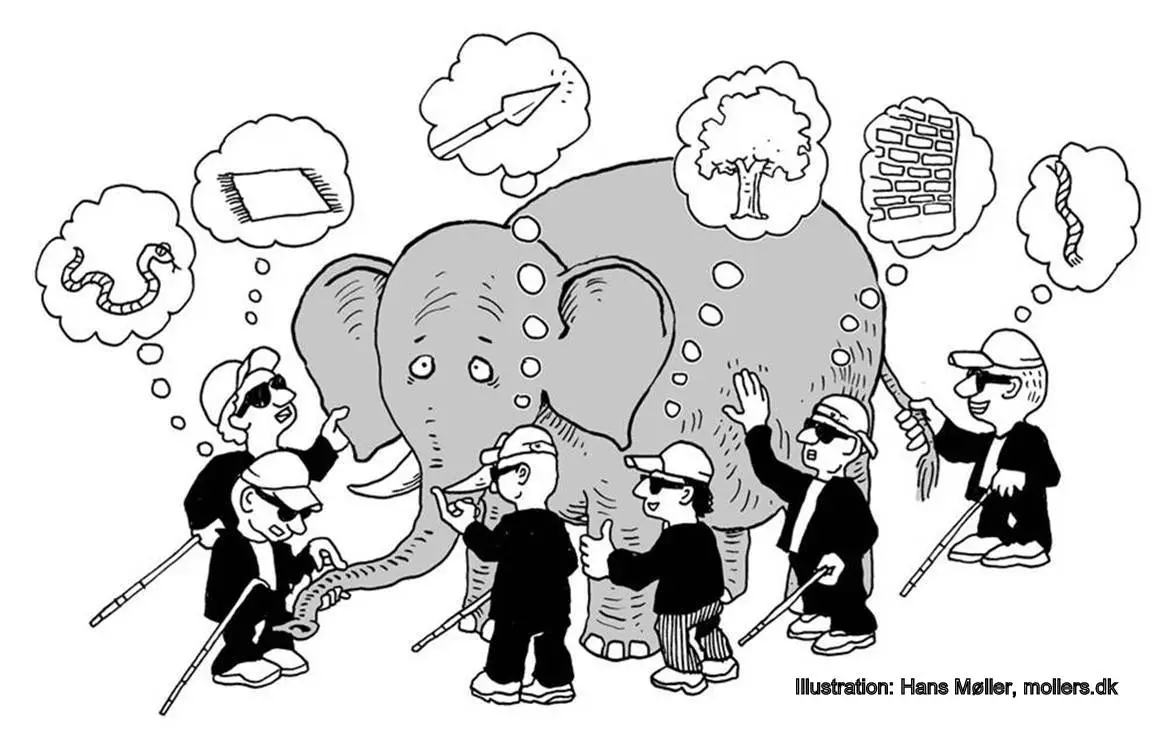
\includegraphics[width=16.17in]{Unidad-I/elefante} 

}

\caption{La parábola de los seis hombres ciegos inspeccionando un elefante.}\label{fig:unnamed-chunk-3}
\end{figure}

Quien toque los colmillos podrá pensar que se trata de una lanza, la trompa podría tratarse de una serpiente, la cola de una cuerda. Es evidente que todas las hipótesis presentadas después de la inspección fueron erróneas, y que cuando estudiamos al mundo lo haremos igual, con la descripción de tan sólo una fracción de éste. Al igual que los ciegos, no sabremos que estmos frente a un elefante, aunque en nuestro caso, en ecología, estudiaremos a un sistema. El elefante, está compuesto de sus partes (orejas, cola, extremidades, piezas dentales) las cuales están conectadas y hacer que el elefante funcione como uno solo, los sistemas ecológicos también tienen componentes interconectados. Así llegamos a la definición de sistema, el objeto de estudio de la ecología, y las matemáticas, son una manera de representarlos

Los hombres ciegos de la parábola, enombraron una hipótesis sobre la identidad del objeto basados en sus experiencias de vida. Los modelos matemáticos entonces, representan hipótesis sobre cómo creemos que los sistemas ecológicos funcionan. Podemos entonces ver que al igual que los ciegos, si sólo nos enfocamos en un aspecto aislado del sistema de estudio, es muy probable que nuestra hipótesis sean erróneas.

\hypertarget{cuxf3mo-construir-un-modelo}{%
\section{Cómo construir un modelo}\label{cuxf3mo-construir-un-modelo}}

\hypertarget{discusiuxf3n-sobre-las-distintas-herramientas-matemuxe1ticas-empleadas-en-la-modelaciuxf3n-matemuxe1tica}{%
\section{Discusión sobre las distintas herramientas matemáticas empleadas en la modelación matemática}\label{discusiuxf3n-sobre-las-distintas-herramientas-matemuxe1ticas-empleadas-en-la-modelaciuxf3n-matemuxe1tica}}

\hypertarget{uso-de-los-modelos-matemuxe1ticos-en-ecologuxeda}{%
\section{Uso de los modelos matemáticos en ecología}\label{uso-de-los-modelos-matemuxe1ticos-en-ecologuxeda}}

\hypertarget{tipos-de-modelos-en-ecologuxeda}{%
\section{Tipos de modelos en ecología}\label{tipos-de-modelos-en-ecologuxeda}}

\hypertarget{modelos-deterministas-generalidades}{%
\subsection{Modelos deterministas (generalidades)}\label{modelos-deterministas-generalidades}}

\hypertarget{modelos-estocuxe1sticos-generalidades}{%
\subsection{Modelos estocásticos (generalidades)}\label{modelos-estocuxe1sticos-generalidades}}

\hypertarget{funciones-complementarias-y-su-representaciuxf3n-en-dos-y-tres-dimensiones}{%
\section{Funciones complementarias y su representación en dos y tres dimensiones}\label{funciones-complementarias-y-su-representaciuxf3n-en-dos-y-tres-dimensiones}}

\hypertarget{la-luxednea-recta-como-modelo-universal}{%
\section{La línea recta como modelo ``universal''}\label{la-luxednea-recta-como-modelo-universal}}

\hypertarget{modelaciuxf3n-de-sistemas-sociales-y-ambientales}{%
\section{Modelación de sistemas sociales y ambientales}\label{modelaciuxf3n-de-sistemas-sociales-y-ambientales}}

\hypertarget{methods}{%
\chapter{Methods}\label{methods}}

We describe our methods in this chapter.

\hypertarget{applications}{%
\chapter{Applications}\label{applications}}

Some \emph{significant} applications are demonstrated in this chapter.

\hypertarget{example-one}{%
\section{Example one}\label{example-one}}

\hypertarget{example-two}{%
\section{Example two}\label{example-two}}

  \bibliography{book.bib,packages.bib}

\end{document}
